%-------------------------------------------------------------------------------
%	PACKAGES AND OTHER DOCUMENT CONFIGURATIONS
%-------------------------------------------------------------------------------

\documentclass{article}

% Packages
% Packages

% \usepackage{fancyhdr} % Required for custom headers
% \usepackage{lastpage} % Required to determine the last page for the footer
% \usepackage{extramarks} % Required for headers and footers
% \usepackage[usenames,dvipsnames]{color} % Required for custom colors
\usepackage{graphicx} % Required to insert images
% \usepackage{listings} % Required for insertion of code
% \usepackage{courier} % Required for the courier font
% \usepackage{dsfont} % For special math characters
% \usepackage{verbatim}

%\usepackage{amsmath, amssymb, bm} % For matrix notation
\usepackage[english]{babel}
\usepackage[paperwidth=8.5in,paperheight=11in,margin=1.0in]{geometry}
\usepackage{listings}
\usepackage{hyperref}
%\usepackage[cmex10]{amsmath, bm}
\usepackage{amsmath, bm}
\usepackage{blkarray}








% formatting
\pdfcompresslevel0

% ==============================================================================
% PYTHON
% ==============================================================================
\usepackage[utf8]{inputenc}

% Default fixed font does not support bold face
\DeclareFixedFont{\ttb}{T1}{txtt}{bx}{n}{12} % for bold
\DeclareFixedFont{\ttm}{T1}{txtt}{m}{n}{12}  % for normal

% Custom colors
\usepackage{color}
\definecolor{deepblue}{rgb}{0,0,0.5}
\definecolor{deepred}{rgb}{0.6,0,0}
\definecolor{deepgreen}{rgb}{0,0.5,0}

\usepackage{listings}

% Python style for highlighting
\newcommand\pythonstyle{\lstset{
language=Python,
basicstyle=\ttm,
otherkeywords={self},             % Add keywords here
keywordstyle=\ttb\color{deepblue},
emph={MyClass,__init__},          % Custom highlighting
emphstyle=\ttb\color{deepred},    % Custom highlighting style
stringstyle=\color{deepgreen},
frame=tb,                         % Any extra options here
showstringspaces=false,            % 
breaklines=true
}}


% Python environment
\lstnewenvironment{python}[1][]
{\pythonstyle\lstset{#1}
}
{}

% Python for external files
\newcommand\pythonexternal[2][]{{
\pythonstyle\lstinputlisting[#1]{#2}}}

% Python for inline
\newcommand\pythoninline[1]{{\pythonstyle\lstinline!#1!}}
% ==============================================================================
% ==============================================================================

% Margins
\topmargin=-0.45in
\evensidemargin=0in
\oddsidemargin=0in
\textwidth=6.5in
\textheight=9.0in
\headsep=0.25in

\linespread{1.1} % Line spacing

% Set up the header and footer
\pagestyle{fancy}
\lhead{\hmwkAuthorName} % Top left header
\chead{\hmwkClass\ (\hmwkClassInstructor\ \hmwkClassTime): \hmwkTitle} % Top center head
\rhead{\firstxmark} % Top right header
\lfoot{\lastxmark} % Bottom left footer
\cfoot{} % Bottom center footer
\rfoot{Page\ \thepage\ of\ \protect\pageref{LastPage}} % Bottom right footer
\renewcommand\headrulewidth{0.4pt} % Size of the header rule
\renewcommand\footrulewidth{0.4pt} % Size of the footer rule

\setlength\parindent{0pt} % Removes all indentation from paragraphs

%----------------------------------------------------------------------------------------
%	DOCUMENT STRUCTURE COMMANDS
%	Skip this unless you know what you're doing
%----------------------------------------------------------------------------------------

% Header and footer for when a page split occurs within a problem environment
\newcommand{\enterProblemHeader}[1]{\nobreak\extramarks{#1}{#1 continued on next page\ldots}\nobreak\nobreak\extramarks{#1 (continued)}{#1 continued on next page\ldots}\nobreak}

% Header and footer for when a page split occurs between problem environments
\newcommand{\exitProblemHeader}[1]{\nobreak\extramarks{#1 (continued)}{#1 continued on next page\ldots}\nobreak\nobreak\extramarks{#1}{}\nobreak}

\setcounter{secnumdepth}{0} % Removes default section numbers
\newcounter{homeworkProblemCounter} % Creates a counter to keep track of the number of problems

\newcommand{\homeworkProblemName}{}
\newenvironment{homeworkProblem}[1][Problem \arabic{homeworkProblemCounter}]{ % Makes a new environment called homeworkProblem which takes 1 argument (custom name) but the default is "Problem #"
\stepcounter{homeworkProblemCounter} % Increase counter for number of problems
\renewcommand{\homeworkProblemName}{#1} % Assign \homeworkProblemName the name of the problem
\section{\homeworkProblemName} % Make a section in the document with the custom problem count
\enterProblemHeader{\homeworkProblemName} % Header and footer within the environment
}{\exitProblemHeader{\homeworkProblemName} % Header and footer after the environment
}

% Defines the problem answer command with the content as the only argument
\newcommand{\problemAnswer}[1]{\noindent\framebox[\columnwidth, resolution=600][c]{\begin{minipage}{0.98\columnwidth, resolution=600}#1\end{minipage}}}
% Makes the box around the problem answer and puts the content inside }

\newcommand{\homeworkSectionName}{}
\newenvironment{homeworkSection}[1]{ % New environment for sections within homework problems, takes 1 argument - the name of the section
\renewcommand{\homeworkSectionName}{#1} % Assign \homeworkSectionName to the name of the section from the environment argument
\subsection{\homeworkSectionName} % Make a subsection with the custom name of the subsection
\enterProblemHeader{\homeworkProblemName\ [\homeworkSectionName]} % Header and footer within the environment
}{
\enterProblemHeader{\homeworkProblemName} % Header and footer after the environment
}



%-------------------------------------------------------------------------------
%	NAME AND CLASS SECTION
%-------------------------------------------------------------------------------

\newcommand{\hmwkTitle}{Homework 7} % Assignment title
\newcommand{\hmwkDueDate}{Friday, Nov 7} % Due date
\newcommand{\hmwkClass}{ECE 532} % Course/class
\newcommand{\hmwkClassTime}{11:00 am} % Class/lecture time
\newcommand{\hmwkClassInstructor}{Robert Nowak} % Teacher/lecturer
\newcommand{\hmwkAuthorName}{Elijah Bernstein-Cooper} % Your name

%-------------------------------------------------------------------------------
%	TITLE PAGE
%-------------------------------------------------------------------------------

\title{\vspace{0in}
    \textmd{\textbf{\hmwkClass:\ \hmwkTitle}}\\
    \normalsize\vspace{0.1in}\small{Due\ on\ \hmwkDueDate}\\
    \vspace{0.1in}\large{\textit{\hmwkClassInstructor\ \hmwkClassTime}}
    \vspace{0.5in}}

\author{\textbf{Elijah Bernstein-Cooper}}
\date{\today} % Insert date here if you want it to appear below your name

%-------------------------------------------------------------------------------

\begin{document}

\maketitle
%\newpage

%===============================================================================
%-------------------------------------------------------------------------------
%	PROBLEM 1
%-------------------------------------------------------------------------------
\begin{homeworkProblem}

    We derived dual and primal least squares solutions to classify the training
    data. We set the regularization parameter $\lambda = 10^{-5}$. See
    Figure~\ref{fig:prob1} for the resulting prediction compared to the
    original training data. 50\% of the data was classified incorrectly by
    least squares. See the code at the end of the homework.
    
    \begin{figure}[!ht]
        \begin{centering}
        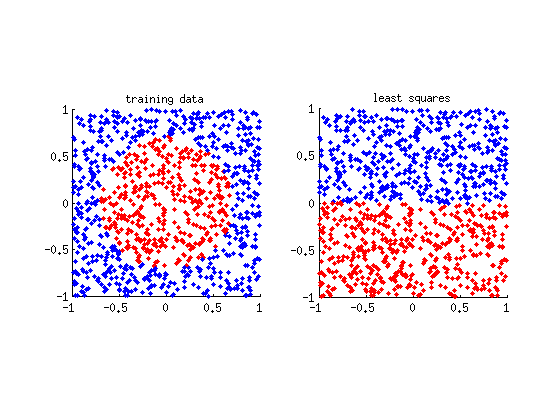
\includegraphics[scale=1.]{fig_prob1.png}

        \caption{\label{fig:prob1} The original data on the left, classified as
            negative (red) or positive (blue). The least squares dual solution
            is shown in the middle, and the least squares primal solution is
            shown on the right. We can see that least squares is an
            inappropriate classifier for this data.}
        \end{centering}

    \end{figure} 

\end{homeworkProblem}
\clearpage
%===============================================================================

%===============================================================================
%-------------------------------------------------------------------------------
%	PROBLEM 2 
%-------------------------------------------------------------------------------
\begin{homeworkProblem}
   
    We classified the training data with a Gaussian kernel, which is a much
    more appropriate classifier than least squares. See Figure~\ref{fig:prob2}
    for the results. The percent of mistakes made using the Gaussian kernel was
    1\%, 50 $\times$ fewer mistakes than least squares. We set the
    regularization parameter $\lambda = 10^{-5}$. See the code at the end of
    the homework. 

    \begin{figure}[!ht]
        
        \begin{centering}
        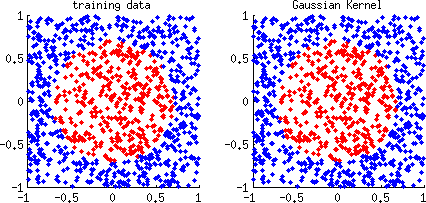
\includegraphics[scale=1.0]{fig_prob2.png}

        \caption{\label{fig:prob2} The original data on the left, classified as
        negative (red) or positive (blue). The Gaussian kernel classification
    is on the right.}
        \end{centering}

    \end{figure} 

\end{homeworkProblem}
%===============================================================================

%===============================================================================
%-------------------------------------------------------------------------------
%	PROBLEM 3
%-------------------------------------------------------------------------------
\begin{homeworkProblem}
   
    We classified the training data with a 2nd order polynomial kernel, which
    is a much more appropriate classifier than least squares, but does not
    perform as well in this case as the Gaussian kernel. See
    Figure~\ref{fig:prob3} for the results. The percent of mistakes made using
    the polynomial kernel was 4\%, 10 $\times$ fewer mistakes than least
    squares, and 4 $\times$ more mistakes than the Gaussian kernel.  We set the
    regularization parameter $\lambda = 10^{-5}$. See the code at the end of
    the homework. 

    \begin{figure}[!ht]
        
        \begin{centering}
        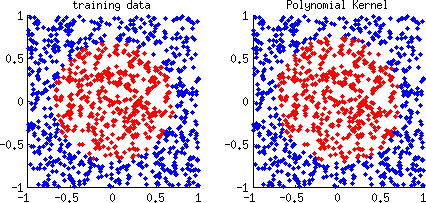
\includegraphics[scale=1.0]{fig_prob3.png}

        \caption{\label{fig:prob3} The original data on the left, classified as
        negative (red) or positive (blue). The polynomial kernel classification
    is on the right.}
        \end{centering}

    \end{figure} 

\end{homeworkProblem}
%===============================================================================

%===============================================================================
%-------------------------------------------------------------------------------
%	PROBLEM 4
%-------------------------------------------------------------------------------
\begin{homeworkProblem}
  
    We performed a simulation of generating datasets of sizes 10$\times$10,
    100$\times$100, 1000$\times$1000. For each dataset size, we ran 100
    iterations of regenerating the data, and classified the generated data with
    the least squares, Gaussian kernel, and polynomial kernels methods. We
    calculated the percent total of mistakes made by each of the three methods,
    see Table~\ref{table:prob4} for the results. See Figure~\ref{fig:prob4} for
    an example of classifications for a 1000$\times$1000 dataset. See the code
    at the end of the homework.

    \begin{table}[!ht]

        \caption{\label{table:prob4} Resulting \% total classification mistakes
        for different methods and dataset sizes.}

        \begin{center}
            \begin{tabular}{lccc}
                
                & 10$\times$10 & 100$\times$100 & 1000$\times$1000 \\
                \hline \hline
                Least Squares     & 33 & 45 & 48.4 \\
                Gaussian Kernel   & 0  & 1 & 1.3 \\
                Polynomial Kernel & 1  & 4 & 3.9 \\

            \end{tabular}
        \end{center}
    \end{table}

    \begin{figure}[!ht]
        
        \begin{centering}
        
        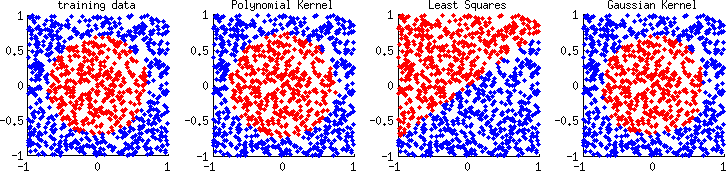
\includegraphics[width=\linewidth]{fig_prob4.png}

        \caption{\label{fig:prob4} Results from classifications of the training
        data. The Gaussian kernel outperforms the least squares and polynomial
    kernel classification.}
        \end{centering}

    \end{figure} 

\end{homeworkProblem}
%===============================================================================

\clearpage
{\huge Code:}

{\large \bf Problem 1} \\
\lstinputlisting{hw7_prob1.m} 
\hrule \hrule

{\large \bf Problem 2} \\
\lstinputlisting{hw7_prob2.m} 
\hrule \hrule

{\large \bf Problem 3} \\
\lstinputlisting{hw7_prob3.m} 
\hrule \hrule

{\large \bf Problem 4} \\
\lstinputlisting{hw7_prob4.m} 
\hrule \hrule

\end{document}

